\chapter{粒子物理标准模型}
由于电弱统一理论和量子色动力学取得的巨大成功，很多人投入到标准模型的构建中去。通常需要场论具有可重整性，不可重整的理论是不自洽的。Wilson重新理解了量子场论中的发散并提出了有效场论的思想，这使得对不同能标处的理论理解更加深刻。本章对量子色动力学进行简单介绍，并基于有效场论的思想介绍重夸克有效理论和基于重夸克有效理论的算符乘积展开，这是后续对粲介子单举半轻衰变做系统性研究的理论基础。

\section{粒子物理标准模型}
\subsection{粒子物理标准模型}
粒子物理标准模型基于规范群
\begin{equation}
    \mathrm{SU}(3)_{\mathrm{C}} \times \mathrm{SU}(2)_{\mathrm{L}} \times \mathrm{U}(1)_{\mathrm{Y}},
\end{equation}
其中，$\mathrm{SU}(3)_\mrm{C}$和$\mathrm{SU}(2)_\mrm{L} $分别是强相互作用和弱相互作用的规范群。一般地，$\mathrm{SU}(2)_\mrm{L} \times \mathrm{U}(1)_\mrm{Y}$自发破缺至描述电磁相互作用的阿贝尔规范群$\mathrm{U(1)_{em}}$; $\mathrm{SU(3)_C}$，$\mathrm{SU(2)_L}$和$\mathrm{U(1)_Y}$的量子数分别是颜色（红绿蓝）、弱同位旋（两个弱同位旋态$T_{3}=\pm\frac{1}{2}$）和超荷（任意实数）。电荷、超荷与弱同位旋的第三分量之间存在以下的关系(Gell-Mann–Nishima relation)，
\begin{equation}
    Q=T_3+Y.
\end{equation}

粒子物理标准模型的物质场可以按照下面两种方式进行分类：按照场在$\mrm{SU}(3)_{\mrm{C}}$规范群变换下的性质，分为夸克和轻子：（反）夸克属于$\mrm{SU}(3)_{\mrm{C}}$的（反）三重态，具有色荷（反）红，（反）绿和（反）蓝，轻子属于$\mrm{SU}(3)_{\mrm{C}}$单态；按照场在$\mathrm{SU(2)_L}$规范群下的变换性质，分为$\mathrm{SU(2)_L}$双重态（左手场）和$\mathrm{SU(2)_L}$单态（右手场），只有$\mathrm{SU(2)_L}$双重态可以参与到弱相互作用带电流。除此之外，标准模型的物质场分为三代，每代之间具有相同的量子数，仅存在质量的差异。

三种局域规范群背后反映了三种局域规范对称性（不变性），局域不变性反过来则要求每个局域规范群都应存在一个属于其自伴表示的无质量规范玻色子。 $\mrm{SU}(3)_{\mrm{C}}$，$\mathrm{SU}(2)_L$和$\mathrm{U}(1)_Y$的无质量规范玻色子分别是属于各自自伴表示的8个胶子、3个$W_{a}^{\mu}$和$B_{\mu}$。电弱对称性破缺之后，$W_{a}^{\mu}$和$B_{\mu}$混合为$W_\mu^{ \pm}, Z^0$ 和 $\gamma$，其中只有光子无质量，对应于描述剩余对称性的阿贝尔规范群$\mathrm{U}(1)_{\mrm{em}}$自伴表示的中间规范玻色子。

在粒子物理标准模型的拉格朗日量涵盖了费米子场的动力学项、规范玻色子的耦合项、希格斯玻色子的动力学项与势能项，以及Yukawa耦合项。规范玻色子的耦合项不仅允许其自身耦合，还通过协变导数算子与费米子场相互耦合。希格斯机制赋予了规范玻色子质量，而希格斯玻色子则通过Yukawa耦合为费米子场提供了质量。

虽然标准模型成功描述了实验现象并且关于新的实验现象的预言不断得到证实，为理解基本粒子之间的相互作用提供了重要的信息。但也有很多悬而未决的问题，比如标准模型没有包含引力相互作用，无法解释正反物质不对称等等，表明粒子物理标准模型并非是最终理论，物理学家也在不断寻找超出标准模型的新物理，以期对宇宙有更深刻、简洁的认识。
\subsection{量子色动力学}
描述夸克和胶子间强相互作用的理论称为量子色动力学（Quantum Chromodynamics, QCD）。尽管由于当前理论精度的限制，量子色动力学尚未能够像量子电动力学那样实现对物理现象的高精度预言，但新物理效应尚未被发现，似乎表明量子色动力学仍具有强大的预言能力。与电弱相互作用不同，量子色动力学严格服从$\mrm{SU(3)_C}$局域规范群对应的颜色规范对称性，因此可以构造出局域规范不变的拉格朗日量，
\begin{equation}
    \mathcal{L}_{\mathrm{QCD}} = \bar{q}_i \left(i \gamma^\mu \partial_\mu \delta_{ij} - g_s \gamma^\mu T_{ij}^a \mathcal{A}_\mu^a - m_q \delta_{ij}\right) q_j - \frac{1}{4} G_{\mu \nu}^a G_a^{\mu \nu},
    \label{eq:QCD_l}
\end{equation}
其中 $\bar{q}_i\left(q_j\right)$ 是带有色指标的反夸克场（夸克场），夸克场的味道 $q=(u, d, s, c, b, t)$ ，其质量是 $m_q$, $\mathcal{A}_\mu^a$ 是带有色指标$a$的胶子场，$a$的取值为从1到8，对应于8种颜色的胶子场，它们属于$SU(3)_C$群的自伴表示。 $T_{ij}^a$是$SU(3)_C$群自伴表示的生成元。$G_{\mu \nu}^a=\partial_\mu \mathcal{A}_\nu^a-\partial_\nu \mathcal{A}_\mu^a-g_s f^{a b c} \mathcal{A}_\mu^b \mathcal{A}_\nu^c$是胶子的规范场强张量。

强相互作用耦合常数$\alpha_s=g_s^2/(4\pi)$具有能标依赖，其满足重整化群方程，
$$
p \frac{\partial}{\partial p} \alpha_\mrm{s}=\beta(p),
$$
区别于量子电动力学， QCD 的 $\beta$ 函数是负的，这表明强相互作用的耦合常数随着相互作用的动量转移增大而减小。在动量转移 $p$ 很大时，$\alpha_s$ 会变得很小，表明在短距离上耦合很弱，这种现象被称为渐进自由，即对强相互作用的高能区域，微扰论是适用的。
$$
\alpha_\mrm{s}(p)=\frac{1}{\left[1 / \alpha_\mrm{s}(\mu)+\beta_0 \ln \left(p^2 / \mu^2\right)\right]},
$$
其中 $\beta_0$ 正比于 $\beta$ 函数的领头阶项，定义非微扰能标$\Lambda_{\mrm{QCD}}=p e^{-1 / 2 \beta_0 \alpha_\mrm{s}(p)}$,强相互作用耦合常数关于非微扰能标的依赖为：
\begin{equation}
    \alpha_\mrm{s}(p)=\frac{12 \pi}{\left(33-2 N_\mrm{q}\right) \ln \left(p^2 / \Lambda_{\mathrm{QCD}}^2\right)} .
    \label{eq:alpha}
    \end{equation}
其中，$N_{\mrm{q}}$是夸克味道数目。式\eqref{eq:alpha}表明，某个过程的转移动量$p$接近非微扰能标$\Lambda_{\mrm{QCD}}$时，$ \alpha_\mrm{s}(\Lambda_{\mrm{QCD}})$是发散的，表明微扰论于该能标处失效。

这是粒子物理领域内长期存在且引起广泛关注一类问题，即量子色动力学非微扰问题。格点量子色动力学基于第一性原理通过将时空离散化以计算低能标处的物理过程。但是随着格距变小，格子数目增加，所需的计算资源爆炸式增长，寻求理论预言精度与计算资源间的平衡使得很多物理问题的研究受限。

此外，有效理论也经常被用于研究强相互作用非微扰，若物理系统中可以构造出一个无量纲的小量, 则可以构造按照其幂次展开的有效场论. 通常, 这样的小量被选为一个小的能量或动量标度和一个大的能量或动量标度之间的比值，使得可以通过幂次展开进行逐阶计算。 同时, 要求有效场论具有的对称性与完整理论的严格或近似对称性一致, 并通过构造满足这些对称性最普遍的拉氏量,从而保证有效场论的计算结果是模型无关的.

由于微扰展开在高能标处的收敛性极好，因此在高能标处的理论研究相对比较成熟，但对于低能非微扰能区的理论研究相对比较匮乏。不同于B介子或底重子，粲夸克的质量更接近非微扰能区，处于微扰区和非微扰区的交界处。在该能标区域，无论是按量子色动力学强相互作用耦合常数展开的高阶微扰修正还是按粲夸克质量负幂次展开的高阶幂次修正，均具有不可忽略的贡献，因此理解粲强子衰变的动力学机制对于理解量子色动力学非微扰的动力学机制具有启示作用。
\section{重夸克有效理论}
事实上，QCD的拉格朗日量（式\eqref{eq:QCD_l}）包含有严格的对称性和近似对称性；前者主要包括洛伦兹对称性、色规范对称性、正反物质对称性等，后者主要包括：手征对称性和重夸克对称性。粒子物理标准模型中，三种夸克的质量远小于非微扰能标，另外三种夸克质量远大于非微扰能标：
\begin{equation}
    m_{\mrm{u, d, s}} \ll \Lambda_{\mathrm{QCD}} \ll m_{\mrm{c, b, t}} .
    \end{equation}
 u, d, s 夸克被称为轻夸克, 而c, b, t 夸克则被称为重夸克。轻夸克部分存在近似的手征对称性及其自发破缺, 而重夸克部分则有近似的重夸克对称性。

 仅考虑三种轻夸克的拉格朗日量，并忽略其质量项（手征极限），意味着左手费米子场和右手费米子场解耦，对应的拉格朗日量具有$\mrm{SU}(3)_{\mrm{R}}\bigotimes\mrm{SU}(3)_{\mrm{L}}$对称性。手征极限下，拉格朗日量的对称性并非真空或强子谱的对称性，量子色动力学的手征对称性自发破缺至矢量子群$\mrm{SU(3)}$，对应$3^2-1$个无质量Goldstone玻色子是最轻的赝标介子八重态\footnote{由于手征对称性并非严格对称性，因此对应的8个无质量玻色子并非严格质量等于零}。手征近似理论仅适用于轻强子及其相互作用。

 不同于u，d，s夸克，c夸克和b夸克的质量远大于非微扰能标。若研究的物理过程涉及到的能动量标度位于$\Lambda_{\mrm{QCD}}$时，$\Lambda_{\mrm{QCD}}/m_{\mrm{Q}}$可被视为小量（$m_{\mrm{Q}}$是重夸克质量）。可以实现以$\Lambda_{\mrm{QCD}}/m_{\mrm{Q}}$为展开参数进行重夸克质量负幂次展开，其领头阶对应于$m_{\mrm{Q}}\to\infty$的极限，在该极限下存在重夸克对称性（重夸克自旋对称性, 重夸克味对称性）。

重夸克自旋相互作用强度正比于磁矩$$
    \propto \frac{\vec{\sigma} \cdot \vec{B}^a}{m_\mrm{Q}} \xrightarrow{m_\mrm{Q} \rightarrow \infty} 0,$$
    其中，$\vec{\sigma}$ 为重夸克的自旋算符，$\vec{B}^a$ 为色磁场。重夸克的自旋在重夸克极限下退耦。考虑一个包含重夸克的系统，其总角动量包含三部分：重夸克的自旋 $\vec{s}_Q$ ，轻自由度（包括轻夸克和胶子）的自旋 $\vec{s}_q$ 和轨道角动量 $\vec{L}$ ：
$$
\vec{J} = \vec{S}_{\mathrm{Q}} + \vec{L} + \vec{s}_{\mathrm{q}} \equiv \vec{S}_{\mathrm{Q}} + \vec{s}_{\ell}.
$$

在重夸克极限下，由于重夸克的自旋退耦，所以总角动量守恒意味着轻自由度的总角动量\footnote{这里讨论基态介子（重子）} $\vec{s}_{\mrm{\ell}}$守恒，属于同一个自旋多重态的重味强子或重夸克偶素的质量在重夸克极限下是简并的。例如基态粲介子 $\left(\mrm{D}, \mrm{D^*}\right)$ 以及基态底介子 $\left(\mrm{\bar{B}},\mrm{ \bar{B}^*}\right)$.

在只包含一个重夸克的强子中,重自由度与轻自由度相互作用强度在非微扰 QCD 的能标 $\Lambda_{\mathrm{QCD}}$ 量级，即放出或吸收胶子对重夸克的速度带来的改变为
$$
\Delta v=\frac{\Delta p}{m_\mrm{Q}}=\mathcal{O}\left(\frac{\Lambda_{\mathrm{QCD}}}{m_\mrm{Q}}\right) \xrightarrow{m_\mrm{Q} \rightarrow \infty} 0,
$$
即在重夸克极限下, 单重强子内的重夸克是几乎静止的, 其仅作为提供$\mrm{SU}(3)_{\mrm{C}}$色三重态而存在，重费米子场（粲夸克和底夸克）在重夸克极限是简并的。

QCD中重夸克部分的拉格朗日量为：
\begin{equation}
    \mathscr{L}_{\mathrm{Q}} = \bar{Q}\left(i \slashed{D} - m_{\mathrm{Q}}\right) Q, \quad D_\mu = \partial_\mu + i g_\mrm{s} A_\mu^a T^a,
    \label{eq:QCD_heavyquark_l}
\end{equation}

式\eqref{eq:QCD_heavyquark_l}中，包含了关于夸克味道的求和。在QCD中，重夸克的传播子为
\begin{equation}
    \frac{i}{\slashed{p} - m_{\mathrm{Q}} + i \epsilon} = \frac{i\left(\slashed{p} + m_{\mathrm{Q}}\right)}{p^2 - m_{\mathrm{Q}}^2 + i \epsilon},
\end{equation}
    其中，重夸克的动量为$p=m_{\mrm{Q}}v+k$,$v$是重强子的速度，满足$v^2=1$,$k\sim \mathcal{O}\left(\Lambda_{\mathrm{\mrm{QCD}}}\right)$是重夸克的离壳动量。选取重夸克离壳动量与重夸克质量的比值作为展开参数，则上面的传播子变为
    \begin{equation}
        \frac{i\left[m_{\mathrm{Q}}(1+\slashed{p})+\slashed{k}\right]}{2 m_{\mathrm{Q}} v \cdot k + k^2 + i \epsilon} \xrightarrow{m_{\mathrm{Q}} \rightarrow \infty} \frac{1+\slashed{v}}{2} \frac{i}{v \cdot k} + \mathcal{O}\left(\frac{k}{m_{\mathrm{Q}}}\right).
    \end{equation}    
   当$v=\{1,\vec{0}\}$上式的$(1+\slashed{v})/2$作用到狄拉克旋量投影出正粒子，$(1-\slashed{v})/2$则投影出反粒子。重夸克场可以被因子化为
   $$Q(x)=e^{-i m_{Q}v \cdot x}\left[Q_v(x)+\tilde{Q}_v(x)\right],$$
其中，指数部分减除重夸克质量，它重新将重夸克能动量的零点定义为$m_{\mrm{Q}}v$.$\tilde{Q}_v(x)$表示减除重夸克质量之后受到$1/m_{\mrm{Q}}$压低的部分，${Q}_v(x)$则表示领先幂次的部分。
将上式代入QCD拉格朗日量\label{eq:QCD_heavyquark_l}中，并经过必要的化简，得到重夸克有效理论的拉格朗日量
\begin{equation}
    \begin{aligned}
    L & =\bar{Q}_v\left(i v \cdot D+i \slashed{D}_{\perp} \frac{1}{2 m_\mrm{Q}+i v \cdot D} i \slashed{D}_{\perp}\right) Q_v \\
    & =\bar{Q}_v\left(i v \cdot D-\frac{1}{2 m_\mrm{Q}} \slashed{D}_{\perp} \slashed{D}_{\perp}+\cdots\right) Q_v \\
    & =L_0+L_1+\cdots,
    \end{aligned}
    \end{equation}
其中领头阶具有明显的重夸克味道对称性和重夸克自旋对称性，相应的运动方程$i v\cdot D Q_{v}=0$;拉格朗日量按照重夸克展开的次领先幂次，包含$-\bar{Q}_v \frac{D_{\perp}^2}{2 m_\mrm{Q}} Q_v$和$-g \bar{Q}_v \frac{\sigma_{\mu v} G^{\mu \nu}}{4 m_\mrm{Q}} Q_v$，前者破坏了重夸克味道对称性，后者破坏了重夸克味道-自旋对称性，且关于重夸克对称性的破坏受到$1/m_{\mrm{Q}}$的压低。
\section{基于重夸克有效理论的局域算符乘积展开}
由于重夸克质量远大于$\Lambda_{\mrm{QCD}}$，因此对于重强子衰变的物理可观测量，存在按强相互作用耦合常数$\alpha_\mrm{s}$的微扰展开和按$\Lambda_{\mrm{QCD}}/m_{\mrm{Q}}$的幂次展开，这使得逐阶计算成为可能。在B介子与底重子的精确计算中，这样的双重展开具有极好的收敛性。但在D介子与粲重子弱衰变中，其微扰展开与幂次展开的收敛性均存在长期的讨论。

具体地，根据光学定理，某个过程的衰变宽度与该过程向前散射振幅的虚部相关，以$\mrm{D}\to \mrm{X_{s}e^+\nu}$为例(图\ref{fig:HQEc})，
\begin{figure}[h!]
    \centering
    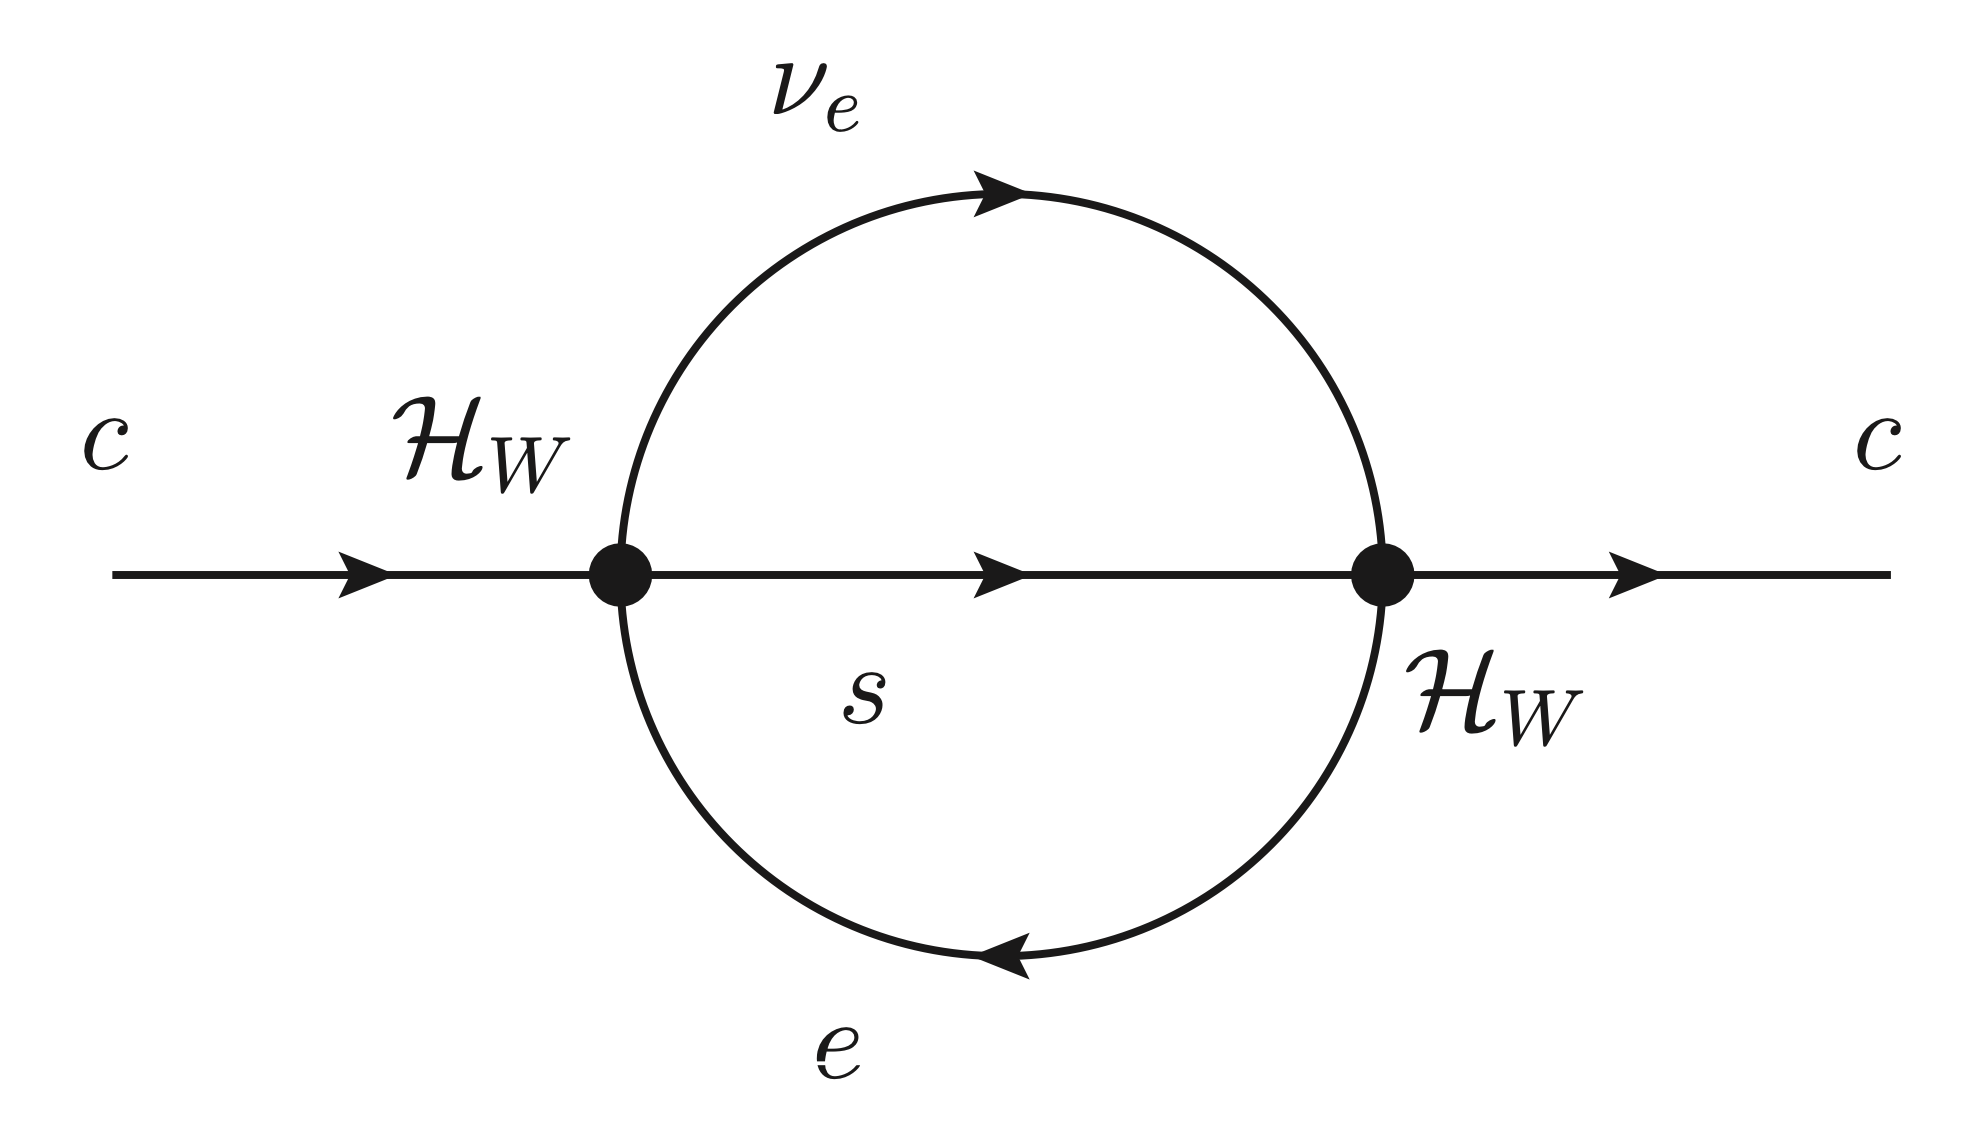
\includegraphics[width=0.4\textwidth]{figures/HQEc.png}
    \caption{算符乘积展开领先幂次贡献\ct{Fael:2019umf}}
    \label{fig:HQEc}
\end{figure}
其衰变宽度为
\begin{equation}
    \Gamma=\frac{1}{\mrm{M}_\mrm{D}} \operatorname{Im}\langle \mrm{D}| i \int \mrm{d}^4 x e^{-i p_\mrm{D} \cdot x} \operatorname{T}\left\{\mathcal{H}_W^{\dagger}(x), \mathcal{H}_W(0)\right\}|\mrm{D}\rangle=\frac{1}{\mrm{M}_\mrm{D}} \operatorname{Im}\langle \mrm{D}| R|\mrm{D}\rangle,
    \label{eq:decaywidth_c}
\end{equation}
其中弱有效哈密顿量为：\begin{equation}
    \mathcal{H}_W=\frac{4 \mrm{G_F}}{\sqrt{2}} \mrm{V_{\mathrm{CKM}}}\left(\mrm{\bar{q}} \gamma_\mrm{L}^\mu \mrm{c}\right)\left(\mrm{\overline{\nu}_{\ell}} \gamma_{\mrm{L} \mu} \mrm{\ell}\right)=\frac{4 \mrm{G_F}}{\sqrt{2}} \mrm{V}_{\mathrm{CKM}} J_\mrm{q}^\mu J_{\mrm{\ell} \mu},
    \end{equation}
其中，$\gamma_{\mathrm{L}}^\mu = \gamma^\mu P_{\mathrm{L}}, \quad P_{\mathrm{L}} = \frac{1 - \gamma_5}{2}$
是左手投影算子，$\mrm{G_{F}}$是费米常数，$\mrm{V}_{\mathrm{CKM}}$是相关的CKM矩阵元模方，$J_\mrm{q}^\mu$ 和 $J_{\mrm{\ell}}^\mu$分别是强子流和轻子流。

式\eqref{eq:decaywidth_c}中的非局域算符的编时乘积可以用一组局域算符展开，
\begin{equation}
    \operatorname{T}\left\{\mathcal{H}_W^{\dagger}(x), \mathcal{H}_W(0)\right\}=\sum C^n(x) \mathscr{O}_n(0).
    \label{eq:OPE}
\end{equation}
其中树图水平上对应的局域算符是两夸克算符，其一般形式为 $\bar{Q}_v\left(i D^{\mu_1} \ldots i D^{\mu_n}\right) Q_v$, $D^{\mu}$是协变微分算子，其本征值为离壳动量$k\sim \Lambda_{\mrm{QCD}}$。 式\eqref{eq:OPE}中,展开系数$C^n(x)$对应于该过程的短程微扰贡献，而受到$1/m_{\mrm{c}}$压低的局域算符矩阵元对应于长程非微扰贡献。前者可以通过微扰理论逐阶计算，后者涉及强相互作用非微扰，需要通过格点量子色动力学或从实验数据中抽取得到。

计算$\mrm{c}\to \mrm{s} e^+\nu$过程分为三步：首先在微扰展开的特定阶，在$\mu\sim m_{\mrm{c}}$处抽取出Wilson系数。由于算符乘积展开是算符之间的关系，可以通过将式\eqref{eq:OPE}置于夸克和胶子态中，计算Wilson系数；其次，Wilson系数必须通过求解对应局域算符的反常量纲并通过重整化群方程演化到$\mu<m_{\mrm{c}}$处；最后，衰变宽度可以用一组局域算符矩阵元（非微扰参数）进行参数化，一般标记为$\mrm{X}_i(\mu)$，
\begin{equation}
    \left.2 M_\mrm{D} \mrm{X}_i(\mu) \equiv\langle \mrm{D}| O_i|\mrm{D}\rangle\right|_\mu.
    \end{equation}
对于D介子半轻单举衰变过程，通常非局域算符通常可以用以下一组局域算符\ct{Fael:2019umf}进行展开\footnote{精确至量纲七算符}，
\begin{equation}
    \begin{array}{ll}
    O_{\mu_3}=\bar{c}_v c_v, & O_{r_G}=\bar{c}_v\left[\left(i D_\mu\right),\left(i D_\nu\right)\right]\left[\left(i D^\mu\right),\left(i D^\nu\right)\right] c_v, \\
    O_{\mu_\pi}=\bar{c}_v(i D)^2 c_v, & O_{r_E}=\bar{c}_v\left[(i v D),\left(i D_\mu\right)\right]\left[(i v D),\left(i D^\mu\right)\right] c_v, \\
    O_{\mu_G}=\bar{c}_v \sigma \cdot G c_v, & O_{s_B}=\bar{c}_v\left[\left(i D_\mu\right),\left(i D_\alpha\right)\right]\left[\left(i D^\mu\right),\left(i D_\beta\right)\right]\left(-i \sigma^{\alpha \beta}\right) c_v, \\
    O_{\rho_D}=\frac{1}{2} \bar{c}_v\left[i D^\mu,\left[i v D, i D_\mu\right]\right] c_v, & O_{s_E}=\bar{c}_v\left[(i v D),\left(i D_\alpha\right)\right]\left[(i v D),\left(i D_\beta\right)\right]\left(-i \sigma^{\alpha \beta}\right) c_v, \\
    O_{\delta \rho_D}=\frac{1}{2} \bar{c}_v\left[i D^\mu,\left[(i D)^2, i D_\mu\right]\right] c_v, & O_{s_{q B}}=\bar{c}_v\left[i D_\mu,\left[i D^\mu,\left[i D_\alpha, i D_\beta\right]\right]\right]\left(-i \sigma^{\alpha \beta}\right) c_v,
    \end{array}
    \end{equation}
其中，$\sigma \cdot G \equiv-i \sigma^{\mu \nu}\left(i D_\mu\right)\left(i D_\nu\right)$，$\sigma^{\mu \nu}=\frac{i}{2}\left[\gamma^\mu, \gamma^\nu\right]$.最终$\mrm{D}\to \mrm{X}_{\mrm{s}}e^{+}\nu$过程的半轻单举衰变宽度用该组局域算符的非微扰矩阵元参数化为
\begin{equation}
    \begin{aligned}
    \frac{\Gamma\left(\mathrm{D} \rightarrow \mathrm{X}_{\mathrm{s}} \ell \nu\right)}{\Gamma_0} & = \left(1 - 8 \rho - 10 \rho^2\right) \mu_3 + (-2 - 8 \rho) \frac{\mu_\mrm{G}^2}{m_\mrm{c}^2} + 6 \frac{\tilde{\rho}_\mrm{D}^3}{m_\mrm{c}^3} \\
    & + \frac{16}{9} \frac{r_\mrm{G}^4}{m_\mrm{c}^4} + \frac{32}{9} \frac{r_\mrm{E}^4}{m_\mrm{c}^4} - \frac{34}{3} \frac{s_\mrm{B}^4}{m_\mrm{c}^4} + \frac{74}{9} \frac{s_\mrm{E}^4}{m_\mrm{c}^4} + \frac{47}{36} \frac{s_{\mathrm{qB}}^4}{m_\mrm{c}^4} + \frac{\tau_0}{m_\mrm{c}^3},
    \end{aligned}
\end{equation}
%其中，$\rho=m_s^2 / m_c^2$, $\Gamma_{0}=\frac{G_F^2m_{c}^5|V_{cs}|^2}{192\pi^3}$。

本文将讨论D介子半轻单举衰变过程中的物理可观测量的构造，其依赖于这些局域算符的非微扰强子矩阵元；与此同时，从实验数据中抽取出相应物理可观测量的实验观测值，与理论表达式一起进行全局拟合以期实现对局域算符非微扰强子矩阵元的拟合抽取；D介子半轻衰变与非轻衰变的不同之处仅在于其Wilson系数不同，因此本文关于局域算符非微扰强子矩阵元的拟合估计值可直接用于D介子衰变宽度的理论计算。

\section{本章回顾}
本章对粒子物理标准模型和量子色动力学进行简单介绍，此外，对量子色动力学的两种近似对称性（手征对称性和重夸克对称性）进行讨论，基于重夸克对称性，讨论了重夸克有效理论和基于重夸克有效理论的算符乘积展开，最终衰变宽度可以用一组局域算符的非微扰矩阵元进行参数化。这是本文对D介子进行系统性研究的理论基础。
